\chapter{The Platform}


\section{Introduction to rafMetrics platform}
This theoretical work includes a proof-of-concept software stack including various metrics evaluation for classic and modern computer programs. The software stack is further referred as the "Platform".

The metrics that require data acquisition are based on web crawlers (interrogations as described in WebMonitoring tool), experimental data (gathered by computing and estimating running time computer algorithms for various input size in cloud-based systems) or symbolic calculus(for computing rComplexity calculus and calculating partial derivatives).

Furthermore, a ML-based system is used for estimating rComplexity in the case when the theoretical mapping between the algorithm's function and the rComplexity Class is not known. For better performances, it should be inputted with the classic Big-Theta(for asymptotic behavior) Class or an acceptable classic Big-O Class approximation. However, this platform can approximate a good fitting for algorithms with unknown classic asymptotic behavior.

The process of automatically tailoring a suitable rComplexity Class is provided on-demand, using rafComputing Tool.


\section{Codebase}
All the code can be accessed and used via GitHub at \href{https://github.com/raresraf/rafMetrics}{https://github.com/raresraf/rafMetrics}.
\\
rafMetrics is licensed under the MIT License: a short and simple permissive license with conditions only requiring preservation of copyright and license notices. Licensed works, modifications, and larger works may be distributed under different terms and without source code.
\\
An easy-to-use, dockerized implementation, can be found at DockerHub within raresraf/ repositories.


\section{Technologies}

\subsection{Backend}
The main Platform engine is written in Python3, an interpreted, high-level, general-purpose programming language. \\

The WebMonitoring tool and the Login service have been created using Flask framework for a quick and easy API definition. The connection between the Platform and the mySQL database is provided by the official mySQL connectors provided in the mysql-connector-python packages.

For WebMonitoring tool we use thind-party browsers and software applications, including Chrome Driver, a Selenium server or Browsermob-proxy.

The repositories contains few easy deployment scripts that are written in Python or Shell Scripting.

Some mySQL functions and procedures are generated using the build-in rendering Python options.

rafComputing accommodate both an API definition under Flask technology, while the actual Engines for computing and estimating rComplexity are developed using NumPy library.

For time bug-free code a third-party library is used, arrow. This is a Python library that offers a sensible and human-friendly approach to creating, manipulating, formatting and converting dates, times and timestamps.

For monitoring BE an open source analytic \& monitoring solution for the database is desired. Such an implementation is Grafana.

\subsection{Frontend}
The frontend is implemented using React – A JavaScript library for building user interfaces. The platform UI is based on Flatlogic Template: React Material Admin — Material-UI Dashboard. The application can be built using default Node package manager.

\subsection{Deployment}

Each component is containerized using Docker technologies which assures a secure build and unbounded sharing options.

In order to perform a deployment of the Platform as an assembly, few orchestration systems can be used, including Docker Swarm or Kubernetes.


\section{Networking}

Networking is performed inside the orchestrator using an overlay network managed by Docker Swarm or Kubernetes services with static ClusterIPs and NodePorts.

Docker's overlay networks implementations connect multiple Docker machines and allow swarm services to communicate with each other, facilitating communication between two containers running on
different docker swarm nodes.

In Kubernetes, there are four distinct networking problems to address ~\cite{authors2017kubernetes}:

\begin{itemize}
    \item Highly-coupled container-to-container communications: this is solved by pods and localhost communications.
    \item Pod-to-Pod communications: every Pod gets its own IP address
    \item Pod-to-Service communications: this is covered by Kubernetes services.
    \item External-to-Service communications: this is covered by Kubernetes services.
\end{itemize}

The default node port range for Kubernetes is 30000 - 32767.


\section{Architecture}

\subsection{Architecture overview}


\begin{figure}[H]
    \centering
    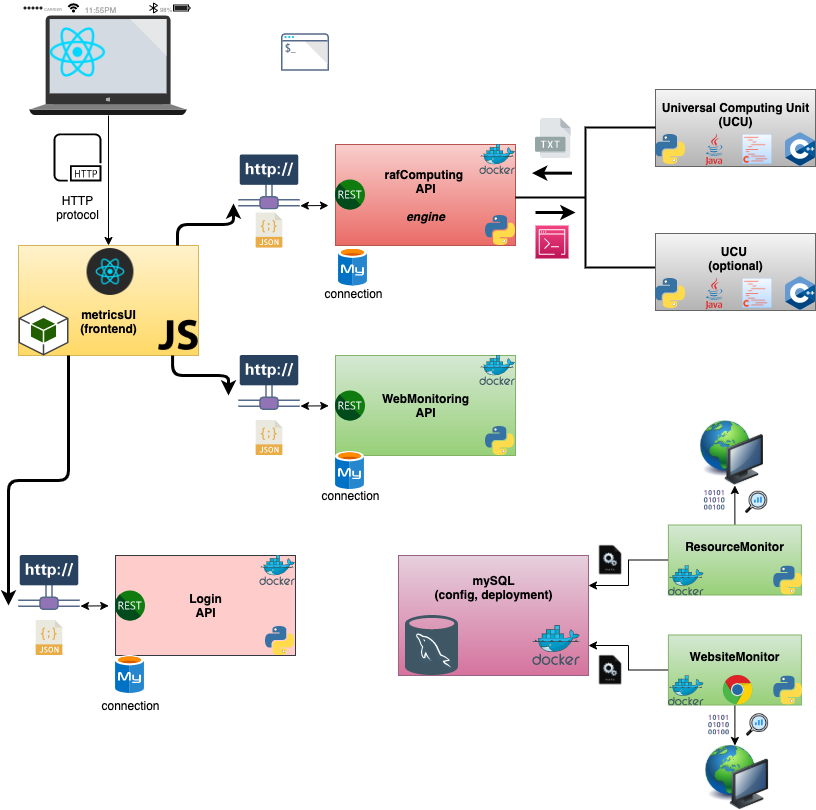
\includegraphics[width=1\textwidth]{arch}
    \caption{An overview of the architecture of the rafMetrics' platform}
\end{figure}

\subsection{Components}
The platform is made up of the following components:

\subsubsection{rafComputing}
The ML-based tool implementing the process of automatically tailoring a suitable rComplexity Class for an algorithm.


A suitable rComplexity Class set is defined by the group of mathematical functions similar in magnitude with  $g(n)$ in the study of asymptotic behavior. A set-based description of this group can be expressed as:
\[\begin{split}
      \Theta_{1}(g(n)) = \lbrace f \in \mathcal{F}\ |\ \forall c_{1}, c_{2} \in \mathbb{R}^{*}_{+} \ s.t. c_{1} < 1 < c_{2} , \exists n_{0} \in \mathbb{N}^{*}\ \\ s.t.\ \ c_{1} \cdot g(n) \leq f(n) \leq c_{2} \cdot g(n)\ ,\  \forall n \geq n_{0} \rbrace
\end{split} \]

\subsubsection{WebMonitoring}
A tool for monitoring multiple network resources and websites.
Gather data by periodically monitoring specific resources and websites and stores results in database.

The following metrics are defined inner WebMonitoring Tool:
\begin{itemize}
    \item Resource Crunch (known as Resource, part of WebMonitioring Tool): Average Response Time (daily, weekly, monthly, custom), Average Response Size, Lowest, Medium, Median, Highest metric time, Efficiency Metric
    \item Website Crunch (known as Website, part of WebMonitioring Tool): Average Response Time (daily, weekly, monthly, custom), Average Response Size (daily, weekly, monthly, custom)
    \item Statistics Resource Manager: Total time, Total number of Requests, Average Time, Average Size, Standard deviation acquired for last 24 hours or all time.
    \item Statistics Website Manager: Total time, Total number of Requests, Average Time, Average Size, Standard deviation acquired for last 24 hours or all time.
\end{itemize}

\subsubsection{ResourceManager}
Monitors all resources by periodically (timer set default at 1 hour interval) sending requests to existing resources.
Store simple metrics like total time or total requests answer as entries in DB.

\subsubsection{WebsiteManager}
Monitors all websites by periodically (timer set default at 1 hour interval) generating a HAR (HTTP-Archieve data performance file) for loading metrics corresponding to a website, with Chrome using Browsermob-Proxy.
Also parse and store valuable insights resulted from the HAR file into DB.
The service uses [speedprofile](https://github.com/parasdahal/speedprofile) engine.

\subsubsection{WebMonitoring API}
Provide an API for interrogating useful metrics from DB.

The routes defined can be checked in the documentation existing in the codebase.

\subsubsection{Login}
Backend implementation to provide a simple authentication, registration and management for users inside rafMetrics platform.

The routes defined can be checked in the documentation existing in the codebase.

\subsubsection{KubernetesConfig}
Keeps track of all k8s settings.

\subsubsection{DockerConfig}
Keeps track of all Docker Compose/Docker Swarm settings and configurations.

\subsubsection{MySQL}
Database used to store persistent data required by Login and WebMonitoring.
All relations are kept in \textbf{Boyce-Codd Normal Form}.

\begin{figure}[H]
    \centering
    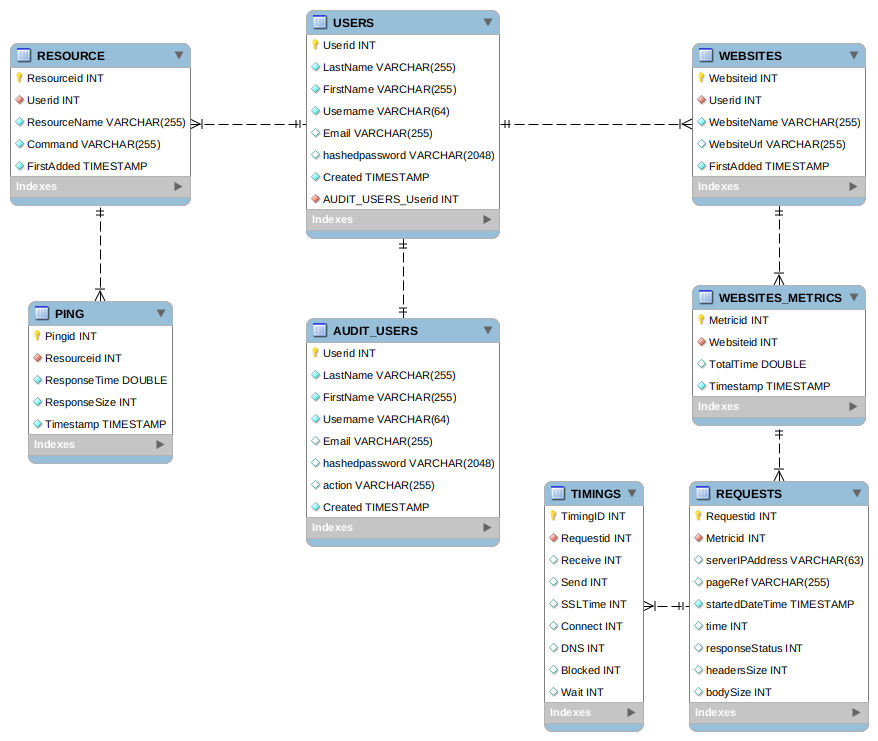
\includegraphics[width=0.7\textwidth]{diagram}
    \caption{SQL table hierarchy used in WebMonitoring Tool}
\end{figure}

The table semantics can be checked in the documentation existing in the codebase.

\subsubsection{deploy\_repo.sh}
Simple script to ensure dockerize and deployment in Kubernetes for all backend components.

\subsubsection{metricsUI}
Frontend implementation of rafMetrics platform based on Flatlogic Template: React Material Admin — Material-UI Dashboard. This component is responsable for rendering UI part of WebMonitoring Tool.

\subsubsection{Grafana}
Grafana ships with a built-in MySQL data source plugin that allow to query any visualize data from a MySQL compatible database.